% % % % % % % % % % % % % % % % % % % % % % % % % % % % % % % %
% import configuration
% % % % % % % % % % % % % % % % % % % % % % % % % % % % % % % %

% % % % % % % % % % % % % % % % % % % % % % % % % % % % % % % %
% Konfiguration
% % % % % % % % % % % % % % % % % % % % % % % % % % % % % % % %
\newcommand{\titleinfo}{Pflichtenheft}
\newcommand{\subjectinfo}{Low Power wakeup receiver}
\newcommand*{\AuthorOne}{Cédric Renda}
\newcommand*{\AuthorTwo}{Manuel Tischhauser}
\newcommand*{\Author}{\AuthorOne, \AuthorTwo}
\newcommand{\authorinfo}{\Author}
\newcommand{\versioninfo}{0.1}
\newcommand{\docNr}{ABC.0001}
\newcommand{\dateinfo}{20.09.2019}

% Notes for SRS completion, uncomment the following command to suppress this output
\newcommand{\note}[1]{%
    \vspace{0.25cm}%
    \colorbox{grey}{%
        \parbox{\linewidth-6pt}{%
            \vspace{0.5cm}%
            \centering%
            \parbox{\linewidth-1cm}{%
                \footnotesize{#1}%
            }%
            \vspace{0.5cm}%
        }%
    }%
    \vspace{0.25cm}}
%\newcommand{\note}[1]{}

% % % % % % % % % % % % % % % % % % % % % % % % % % % % % % % %
% Packages, Layout, Units, etc.
% % % % % % % % % % % % % % % % % % % % % % % % % % % % % % % %
%%%%%%%%%%%%%%%%%%%%%%%%%%%%%%%%%%%%%%%%%%
% Dokument
%%%%%%%%%%%%%%%%%%%%%%%%%%%%%%%%%%%%%%%%%%
% Geometrie
\newcommand{\paperFormat}{a4paper}
\newcommand{\lPageMargin}{20mm}
\newcommand{\rPageMargin}{20mm}
\newcommand{\tPageMargin}{20mm}
\newcommand{\bPageMargin}{20mm}

\documentclass[11pt,oneside]{scrartcl}

\newcommand{\newpar}{\par\par}

\usepackage[pdftitle={\titleinfo},%
			pdfauthor={\authorinfo},%
			pdfcreator={pdfLatex, LaTeX with hyperref},
			pdfsubject={\subjectinfo},
			plainpages=false,
			pdfpagelabels,
			colorlinks,
			linkcolor=black,
			filecolor=black,
			citecolor=black,
			urlcolor=black]{hyperref}
						

% Headings
\usepackage{scrlayer-scrpage}


%%%%%%%%%%%%%%%%%%%%%%%%%%%%%%%%%%%%%%%%%%
% Package's
%%%%%%%%%%%%%%%%%%%%%%%%%%%%%%%%%%%%%%%%%%
\usepackage{ucs}
\usepackage[utf8x]{inputenc}
\usepackage[T1]{fontenc}

\usepackage[free-standing-units=true, use-xspace=true]{siunitx}

\usepackage{layout}
\setlength{\parindent}{0em}

\renewcommand{\baselinestretch}{1.2}
\renewcommand{\arraystretch}{1}

%Damit \today ein Deutsch Formatiertes Datum zurueckgibt.
\usepackage[ngerman, num, orig]{isodate}
\usepackage[german, ngerman]{babel}
\monthyearsepgerman{\,}{\,}

\usepackage{amssymb,amsmath,fancybox,graphicx,wrapfig,color,lastpage,verbatim,epstopdf,a4wide,tabularx}
\usepackage{wasysym} %Checkboxen
\usepackage[usenames,dvipsnames]{pstricks}
\usepackage{setspace}
\usepackage{epsfig}
\usepackage{pst-pdf}
\usepackage{pst-all}
\usepackage{pstricks-add}
\usepackage{supertabular}
\usepackage[font=small,labelfont=bf]{caption}
\usepackage[font=footnotesize]{subfig}
\usepackage{footnote}
\usepackage{float}
\usepackage{multirow}
\usepackage{pdfpages}
\usepackage{pgf,tikz}
\usepackage{color}
\usepackage{titletoc}

\usepackage[makeroom]{cancel}
\usepackage{array}
\usepackage{trfsigns}
\usepackage{textcomp}

%Querformat
\usepackage{pdflscape}

\renewcommand{\captionfont}{\scriptsize\slshape}
	
\setlength{\unitlength}{1mm}

%Inhaltsverzeichnis
\setcounter{secnumdepth}{4}
\setcounter{tocdepth}{2}

%Geometrie
\usepackage[\paperFormat,left=\lPageMargin,right=\rPageMargin,top=\tPageMargin,bottom=\bPageMargin,includeheadfoot]{geometry}


%%%%%%%%%%%%%%%%%%%%%%%%%%%%%%%%%%%%%%%%%%%%%%%%%%%%%%%%%%%%%%%%
% Environment Numbering
%%%%%%%%%%%%%%%%%%%%%%%%%%%%%%%%%%%%%%%%%%%%%%%%%%%%%%%%%%%%%%%%

%Abbildungsnumerierung anhand Kapitel
\renewcommand{\thefigure}{\arabic{section}.\arabic{figure}}
\makeatletter \@addtoreset{figure}{section} \makeatother

%Gleichungen anhand Kapitel
\AtBeginDocument{\numberwithin{equation}{section}}
\AtBeginDocument{\numberwithin{figure}{section}}
\AtBeginDocument{\numberwithin{table}{section}}


%%%%%%%%%%%%%%%%%%%%%%%%%%%%%%%%%%%%%%%%%%%%%%%%%%%%%%%%%%%%%%%%
% Farben
%%%%%%%%%%%%%%%%%%%%%%%%%%%%%%%%%%%%%%%%%%%%%%%%%%%%%%%%%%%%%%%%
\definecolor{black}{rgb}{0,0,0}
\definecolor{red}{rgb}{1,0,0}
\definecolor{white}{rgb}{1,1,1}
\definecolor{grey}{rgb}{0.8,0.8,0.8}


%%%%%%%%%%%%%%%%%%%%%%%%%%%%%%%%%%%%%%%%%%%%%%%%%%%%%%%%%%%%%%%%
% Einheiten
%%%%%%%%%%%%%%%%%%%%%%%%%%%%%%%%%%%%%%%%%%%%%%%%%%%%%%%%%%%%%%%%


%Spannung
\DeclareMathOperator{\V}{\volt}
\DeclareMathOperator{\mV}{\milli \volt}
\DeclareMathOperator{\uV}{\micro \volt}

%Strom
\DeclareMathOperator{\A}{\ampere}
\DeclareMathOperator{\mA}{\milli \ampere}
\DeclareMathOperator{\uA}{\micro \ampere}
\DeclareMathOperator{\nA}{\nano \ampere}

%Zeit
\DeclareMathOperator{\s}{\second}
\DeclareMathOperator{\ms}{\milli \second}
\DeclareMathOperator{\us}{\micro \second}
\DeclareMathOperator{\ns}{\nano \second}

%Kapazitaet
\DeclareMathOperator{\mF}{\milli \farad}
\DeclareMathOperator{\uF}{\micro \farad}
\DeclareMathOperator{\nF}{\nano \farad}
\DeclareMathOperator{\pF}{\pico \farad}
\DeclareMathOperator{\fF}{\femto \farad}

%Induktivitaet
\DeclareMathOperator{\mH}{\milli \henry}
\DeclareMathOperator{\uH}{\micro \henry}
\DeclareMathOperator{\nH}{\nano \henry}

%Widerstand
\DeclareMathOperator{\MO}{\mega \ohm}
\DeclareMathOperator{\kO}{\kilo \ohm}
\DeclareMathOperator{\mO}{\milli \ohm}
\DeclareMathOperator{\Ohm}{\ohm}
%Strecke
\DeclareMathOperator{\km}{\kilo \meter}
\DeclareMathOperator{\cm}{\centi \meter}
\DeclareMathOperator{\mm}{\milli \meter}

%Frequenz
\DeclareMathOperator{\GHz}{\giga \hertz}
\DeclareMathOperator{\MHz}{\mega \hertz}
\DeclareMathOperator{\Hz}{\hertz}
\DeclareMathOperator{\kHz}{\kilo \hertz}
\DeclareMathOperator{\mHz}{\milli \hertz}

%Leistung
\DeclareMathOperator{\kW}{\kilo \watt}
\DeclareMathOperator{\mW}{\milli \watt}
\DeclareMathOperator{\uW}{\micro \watt}
\DeclareMathOperator{\W}{\watt}

%Kreisfrequenz
\DeclareMathOperator{\rpers}{\radianpersecond}

%DeziBel
\DeclareMathOperator{\dB}{\deci \bel}
\DeclareMathOperator{\dBm}{\deci \bel \milli}

%Bit
\DeclareMathOperator{\Bit}{\text{Bit}}
\DeclareMathOperator{\kBit}{\text{kBit}}
\DeclareMathOperator{\MBit}{\text{MBit}}
\DeclareMathOperator{\Byte}{\text{Byte}}
\DeclareMathOperator{\kByte}{\text{kByte}}
\DeclareMathOperator{\MByte}{\text{MByte}}
\DeclareMathOperator{\ppm}{\text{ppm}}

% % % % % % % % % % % % % % % % % % % % % % % % % % % % % % % %
% Dokument
% % % % % % % % % % % % % % % % % % % % % % % % % % % % % % % %
\begin{document}

% % % % % % % % % % % % % % % % % % % % % % % % % % % % % % % %
% Titelseite
% % % % % % % % % % % % % % % % % % % % % % % % % % % % % % % %
\newgeometry{left=20mm, right=20mm, top=10mm, bottom=10mm}

\hrule
\begin{tikzpicture}[scale=1]
\node[] at(0cm,0) {
\includegraphics[height=1.5cm,trim=0mm 2mm 0cm 0mm, clip]{content/title/HSR_Logo_CMYK.eps}};			
\end{tikzpicture}
\hrule
\begin{center}
   	\vspace*{\stretch{1}}
   	\begin{flushright}
   		\Huge
   		\titleinfo\\
   		\Large
   		Projekt: \subjectinfo\\
   		\large
   		\vspace*{\stretch{0.1}}
   		Version \versioninfo\\
   		\vspace*{\stretch{0.5}}
   		\authorinfo \\			
   	\end{flushright}
   	\vspace*{\stretch{2}}	
   	\newcolumntype{Y}{>{\setlength\hsize{0.2\hsize}\raggedright\arraybackslash}X}
   	\newcolumntype{Z}{>{\setlength\hsize{0.4\hsize}\raggedright\arraybackslash}X}
   	\renewcommand\arraystretch{1.5}
   	\begin{tabularx}{\linewidth}{|X|X|X|}
   		\hline
   		\textbf{Name} & \textbf{Datum} & \textbf{Unterschrift}\\
   		\hline
   		Prof. Dr. Heinz Mathis & & \\
   		\hline
   		Selina Malacarne& & \\
   		\hline
   		Cédric Renda& & \\
   		\hline
   		Manuel Tischhauser& & \\
        \hline
   	\end{tabularx}
\end{center}
\cfoot{}
\vspace*{\stretch{0.5}}	
\hrule
{
    \footnotesize 
    \begin{flushright}
        %Doc\#: \docNr\linebreak
        \dateinfo
    \end{flushright}
}

\restoregeometry
	
% % % % % % % % % % % % % % % % % % % % % % % % % % % % % % % %
% Kopf und Fuszeile aktivieren

\pagestyle{scrheadings}
\KOMAoption{headsepline}{true}
\KOMAoption{footsepline}{true}
\ihead{\footnotesize\normalfont \titleinfo}
\ohead{\footnotesize\normalfont \subjectinfo}
\cfoot{}
\setkomafont{pagenumber}{\normalfont}
\ofoot{\footnotesize\normalfont\pagemark\ von \pageref{LastPage}}
\ifoot{\footnotesize\normalfont\copyright\ HSR Hochschule für Technik Rapperswil 2019}
	
% % % % % % % % % % % % % % % % % % % % % % % % % % % % % % % %
% Inhaltsverzeichnis
% % % % % % % % % % % % % % % % % % % % % % % % % % % % % % % %

	{\linespread{1.0} \tableofcontents}
	\newpage
	
		
% % % % % % % % % % % % % % % % % % % % % % % % % % % % % % % %
% Kapitel
% % % % % % % % % % % % % % % % % % % % % % % % % % % % % % % %
	\newpage
		
	%damit " kein umlaut erzeugt und als Anführungszeichn verwendet werden kann
	\shorthandoff{"} %Abschalten mit\shorthandon{"}
    
    % Abbildungen
    %\listoffigures
    %\addcontentsline{toc}{subsection}{Abbildungsverzeichnis}
        
    % Tabellen
    %\listoftables
    %\addcontentsline{toc}{subsection}{Tabellenverzeichnis}
			
	%Includes	
	\section{Einleitung}
\label{sec:intro}

Im Gebäudemanagement ist es üblich, Belegungspläne an den Eingängen der Räume anzubringen.
Oftmals sind diese in Papierformat und müssen bei einer Änderung von Hand gewechselt werden.
Mit dieser Methode werden kurzfristige Belegungen nicht aufgezeigt.
Dies könnte man umgehen, wenn man mit Displays arbeitet, die über eine drahtlose Schnittstelle aktualisiert werden können.
Dabei stellt sich allerdings das Problem, dass man entweder Kabel für die Netzeinspeisung verlegen muss, oder Batterien verwendet, die regelmässig ersetzt werden müssen.
Im Idealfall entfällt die Speisung komplett.
	\section{Auftrag}
\label{sec:generalProvision}

Im Rahmen dieser Semesterarbeit sollen folgende Punkte abgearbeitet werden:
\begin{itemize}
	\item Recherche bezüglich Schnittstelle und Energy Harvesting.	
	\item Vor- und Nachteile bestehender Technologien abwägen und geeignete Hardware wählen.	
	\item Erstellen eines lauffähigen Prototypen.
\end{itemize}

\begin{figure}[h]
	\centering
	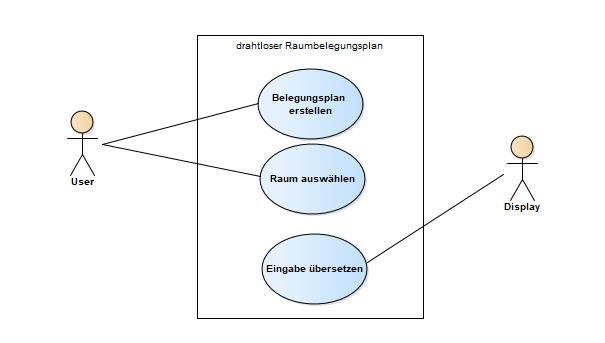
\includegraphics[width=0.8\textwidth]{./Use-Case-Model.png}
	\caption{Use-Case Diagramm\label{use-case}}
\end{figure}

Der Prototyp richtet sich nach dem Use-Case Diagramm in Abbildung \ref{use-case}.
	\section{Produktanforderungen}
\label{sec:funcReqs}
Das Empfängermodul ist autark und kann auf einem Display Stundenpläne anzeigen.
Diese werden über eine drahtlose, bidirektionale Schnittstelle gesendet.
Der Sender wird mit einem Computer bedient.
Besteht das System aus mehreren Empfängern, so kann das Sendemodul diese unabhängig voneinander selektieren.

\subsection{Hardware}
\textbf{Sender}
	\begin{itemize}
		\item[-] Schnittelle zum Computer
		\item[-] Sendemodul
	\end{itemize}

\textbf{Empfänger}
	\begin{itemize}
		\item[-] Mikrocontroller oder Vergleichbares (Prozessor, Speicher, usw.)
		\item[-] E-Paper-Display
		\item[-] Energy-Harvesting-Einheit
		\item[-] Energiespeicher
		\item[-] Empfangsmodul
	\end{itemize}

\subsection{Software}
\textbf{Sender}
\begin{itemize}
	\item[-] Treiber für Sendemodul
\end{itemize}

\textbf{Empfänger}
\begin{itemize}
	\item[-] Firmware für Mikrocontroller
\end{itemize}

\subsection{Varianten/Optionen}
Ist der Prototyp funktionsfähig, soll zu einem späteren Zeitpunkt auch möglich sein, verschiedene Bildschirmgrössen zu verwenden, wobei sich auch Anzeige nicht nur auf Raumbelegungspläne beschränkt.
Deshalb soll das System und insbesondere die Software so flexibel wie möglich entwickelt werden.

\subsection{Dokumentation}
Die Dokumentation beinhaltet sämtliche Überlegungen, Abklärungen, Berechnungen und Untersuchungen, welche im Laufe der Semesterarbeit gemacht wurden.
	%\section{Sonstige Anforderungen}
\label{sec:otherReqs}
\note{In diesesm Kapitel sollen alle bisher noch nicht spezifizierten Anforderungen, möglicherweise in Unterabschnitten, definiert werden, z.B.

\begin{itemize}
\item Leistungsanforderungen (Performance), die nicht direkt einer Systemfunktion zugeordnet werden konnten.
\item Entwurfseinschränkungen (Design Constraints): Anforderungen, welche die Entwickler bei der Wahl des Designs einschränken.
\item Qualitätsanforderungen wie Zuverlässigkeit, Verfügbarkeit, Sicherheit (Safety und Security, ist nicht dasselbe!)
\item Wartbarkeit
\item Portabilität
\item Logging und Tracing
\item Service und Support
\end{itemize}
}


	\begin{landscape}
	\section{Zeitplan}
	\begin{minipage}{23cm}
		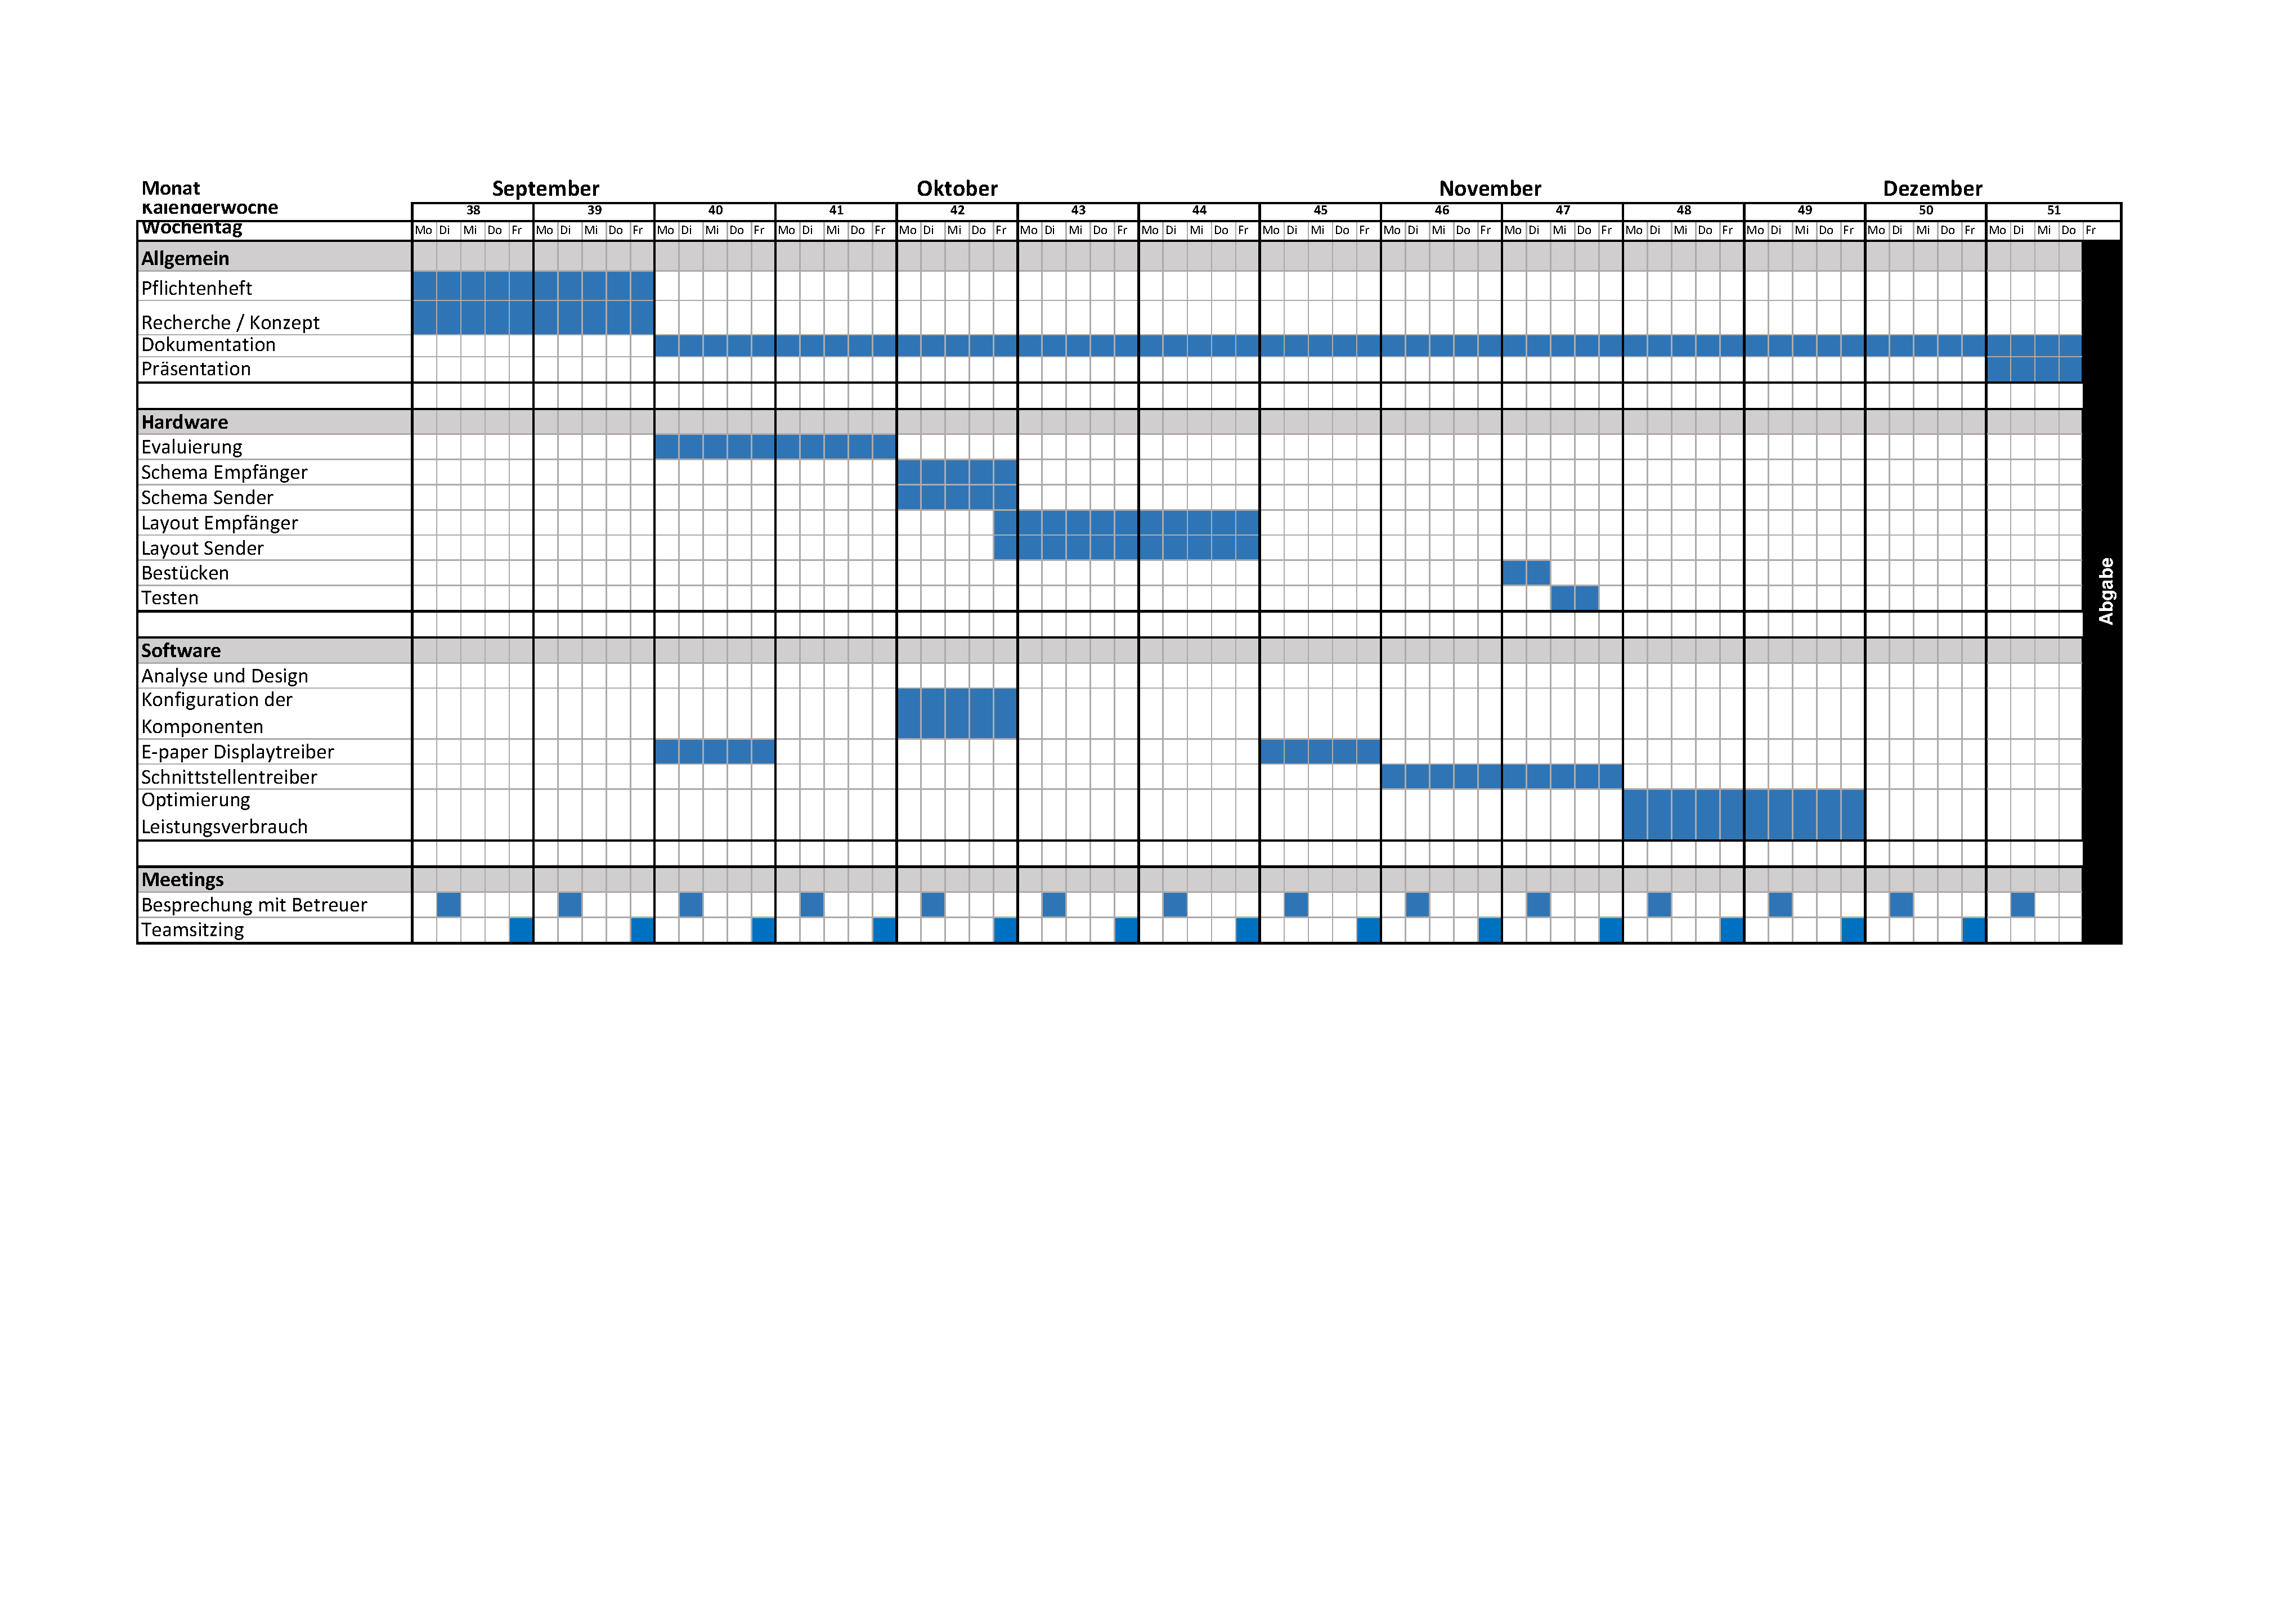
\includegraphics[width=23cm]{./Zeitplan.pdf}
	\end{minipage}	
\end{landscape}
	
% % % % % % % % % % % % % % % % % % % % % % % % % % % % % % % %
% ANHANG
% % % % % % % % % % % % % % % % % % % % % % % % % % % % % % % %
	\appendix
	
	%Nummerierung wieder auf roemisch umschalten
	\newpage
	
	%\section{Referenzen}
	\label{anx:ref}
	% Do not repeat items covered in other documents or in a global project definitions and acronyms document
	%\renewcommand{\refname}{} %kein Titel vor Literaturverzeichnis
	%\vspace{-1.2cm}
	%\bibliographystyle{plain} %Literatur durchnumerieren
	%\bibliography{lit}
	%\nocite{*} %Alle Literatur aufführen
	
	
\end{document}